Đầu tiên các bạn sẽ được làm quen với lý thuyết về đạo hàm.

\textbf{Đạo hàm} của hàm số $f$ tại giá trị $a$, kí hiệu bởi $f'(a)$, là
    \begin{equation}
        f'(a)=\lim_{\Delta x\rightarrow 0}\frac{f(a+\Delta x)-f(a)}{\Delta x}
    \end{equation}
nếu giới hạn này tồn tại.

Đạo hàm còn có ý nghĩa là độ dốc của đồ thị, thể hiện tốc độ biến thiên của hàm số.

\begin{figure}[H]
\centering
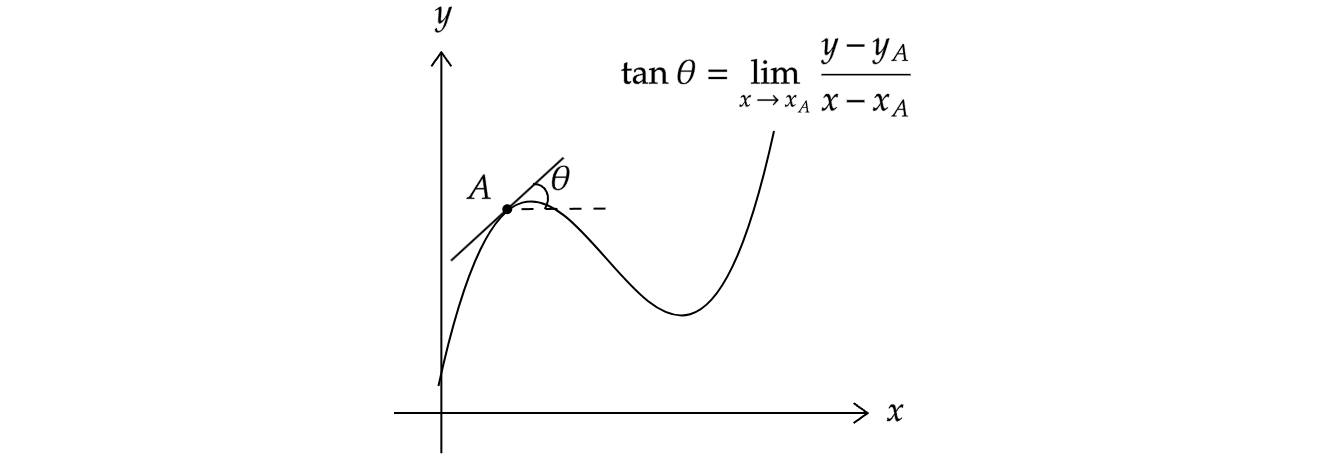
\includegraphics[width=1\textwidth]{Tuan1/Figures/tocdobienthien.png}
\caption{Liên hệ giữa đạo hàm và độ dốc của đồ thị}
\end{figure}
Ở lân cận điểm $x=a$, đồ thị hàm số gần giống với tiếp tuyến của nó tại điểm đó:
\begin{equation}
        f(x)\approx f(a)+f'(a)(x-a)
    \end{equation}
đây được gọi là \textbf{xấp xỉ tuyến tính}.

\textbf{Vi phân} $dy$ của hàm số $y=f(x)$ được xác định theo vi phân $dx$:
\begin{equation}
    dy=f'(x)dx
\end{equation}
và \textbf{phép lấy vi phân} trên có ý nghĩa hình học như hình vẽ:

\begin{figure}[H]
\centering
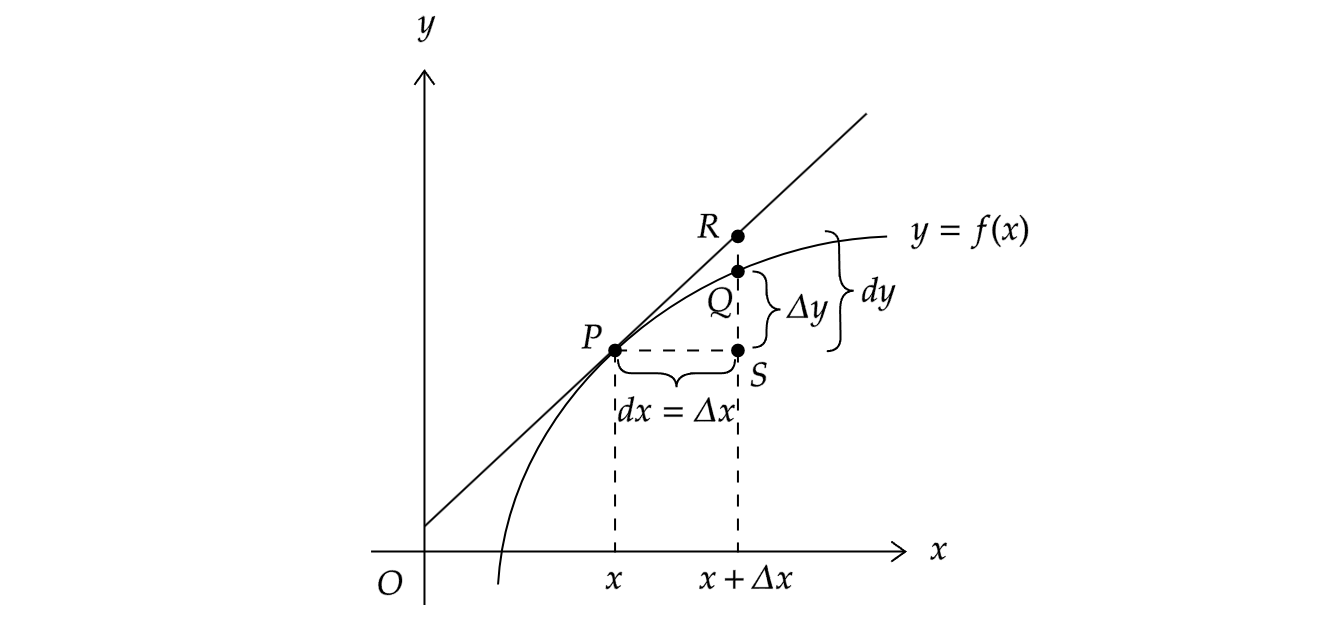
\includegraphics[width=1\textwidth]{Tuan1/Figures/viphan.png}
\caption{Ý nghĩa hình học của phép lấy vi phân}
\end{figure}

Một ví dụ Vật Lý về đạo hàm thường thấy là chuyển động một chiều. Một vật có độ rời $x(t)$ sẽ có vận tốc $v(t)=x'(t)$ và gia tốc $a(t)=x''(t)$.